\ProvidesFile{ch1.tex}[Chapter1]

\chapter{Single molecule localization microscopy}
\ix{physics//Physics appendix}

\section{Introduction}

\subsection{Breaking the diffraction barrier}

In the quest to understand cellular function, biologists aim to directly observe the processes enabling cells to maintain homeostasis and respond dynamically to internal and environmental cues at the molecular level. However, the inherent limitations imposed by diffraction have historically constrained the resolution achievable with conventional light microscopy. The diffraction limit, first described by Ernst Abbe in the 19th century, dictates that the resolution of a microscope is fundamentally limited by the wavelength of light used for imaging. This means that objects closer than approximately half the wavelength of light cannot be distinguished as separate entities. For visible light, this translates to a resolution limit of about 200-250 nanometers, which is insufficient for resolving many subcellular structures and molecular complexes.

Super-resolution (SR) microscopy techniques have emerged as a pathway to observing subcellular structures and dynamics with enhanced resolution, surpassing the classical Abbe diffraction limit: $\lambda/2\mathrm{NA}$ where $\lambda$ is the emission wavelength and $\mathrm{NA}$ is the numerical aperture of an objective lens. Fluorescence microscopy techniques continually push the resolution boundary towards nanometer scales, facilitating imaging of cellular structures with a level of detail previously achievable only with electron microscopy. Concurrently, SR techniques retain optical microscopy advantages in biological experiments, including sample preservation, imaging flexibility, and target specificity. SR enables extraction of quantitative information on spatial distributions and often absolute numbers of proteins, nucleic acids, or other macromolecules within subcellular compartments. \parencite{Kong2013}

A host of SR methods have been developed in recent years, which fundamentally differ in how fluorescently labeled samples are excited and how the emitted photons are detected. Here, I focus on single-molecule localization microscopy (SMLM), also called nanoscopy, techniques. This class of diffraction-unlimited SR methods leverage fluorescence intermittency to resolve fluorophores in the sample who’s spatially overlapping point spread functions would otherwise render them unresolvable at the detector. Nanoscopy approaches, such as direct-STORM (dSTORM) have become quite popular because they can be implemented at low cost on conventional, camera-based, wide-field setups, shifting the complexity to biological sample preparation and image post processing. Common strategies for the temporal separation of molecules involve transient intramolecular rearrangements to switch from dark to fluorescent states or the exploitation of non-emitting molecular radicals. For example, in dSTORM, rhodamine derivatives can undergo intersystem crossing to a triplet state, which can be reduced by thiols to form a dark radical species. The dark state can then be quenched by oxidative processes, driving the fluorophore back to its ground state. 

In nanoscopy applications, we seek the position and intensity of isolated fluorophores as well as to estimate the accuracy and precision of these parameters. Accuracy is a measure of the systematic error or bias, and precision is a measure of the statistical error of an estimator. To generate super-resolution images using SMLM, single emitters are located, and using the mosaic of their found positions, we produce a kernel density estimate (KDE). Such KDEs are often Gaussian, and are used to generate the final super-resolution images. The width of one such placed Gaussian function, $\sigma$ is given by the precision of the fluorophore position localization. Therefore, in SMLM, it is necessary to both find the parameters and estimate their precision. Reported values are in the range of 20–70 nanometers. In the following section, we derive a fundamental statistical description of fluorophore detection in SMLM, which is compatible with a coherent state of the quantized electromagnetic field. This description is necessarily simplified - background rates of light detection may vary across the field of view, and the fluorophore emission rate of chemically identical fluorophores can vary owing to effects such as uneven illumination profile, dipole orientation or different optical path lengths.

\subsection{Biological discovery with fluorescence nanoscopy}

The emergence of fluorescence nanoscopy has marked a significant leap forward in cell biology, enabling researchers to visualize cellular structures with unprecedented clarity and detail. This technological advancement has broken through the limitations of traditional light microscopy, which is constrained by the diffraction limit of light. As a result, scientists can now explore the nanoscale organization of cells and their components, leading to groundbreaking discoveries and new insights into cellular processes.

In the early stages, most nanoscopy studies focused on mammalian cells cultured on flat surfaces, which provided a controlled environment for imaging. These initial studies revealed intricate details of cellular structures, such as organelles and protein complexes, that were previously obscured by the diffraction limit. However, as nanoscopy techniques evolved, researchers began to extend their investigations to more complex and biologically relevant systems. One significant advancement has been the application of nanoscopy to 3D cell cultures, which better mimic the in vivo environment compared to traditional 2D cultures. This has allowed scientists to study cellular interactions and spatial arrangements in a more realistic context. For example, researchers have used nanoscopy to examine the organization of cells within tissue constructs and to investigate the architecture of tissue microenvironments, providing new insights into tissue development and disease.

In immunology, nanoscopy has been employed to study the spatial organization of immune receptors and signaling molecules on the surface of immune cells. This has revealed new insights into how immune cells recognize and respond to pathogens. For example, super-resolution imaging of T-cell receptors has shown how these molecules cluster upon activation, providing a better understanding of the immune response at a molecular level. Nanoscopy has also proven invaluable in microbiology and virology. In these fields, researchers have utilized super-resolution imaging to visualize the structures of viruses and bacteria with exceptional detail. This has led to a deeper understanding of the molecular mechanisms underlying microbial infections and has provided insights into the structure of viral capsids and bacterial surface structures. Such information is critical for developing new antiviral and antibiotic therapies. 

The ability to study cellular structures at the nanoscale has also advanced our understanding of molecular machines and complexes within cells. For instance, detailed imaging of the nuclear pore complex, a crucial structure for nucleocytoplasmic transport, has revealed the precise arrangement of its constituent proteins. This has enhanced our knowledge of how the nuclear pore complex regulates the passage of molecules between the nucleus and cytoplasm, a process essential for cellular function. In cancer biology, nanoscopy has facilitated the investigation of tumor cells and their microenvironment with unprecedented resolution. Researchers have used super-resolution techniques to study the distribution of cancer-related proteins and to understand the spatial organization of tumor cells. This has led to the identification of new biomarkers and potential therapeutic targets, offering hope for more effective cancer treatments.

As nanoscopy continues to evolve, future advancements are likely to enhance both the resolution and speed of imaging, allowing researchers to capture dynamic processes within living cells in real time. New techniques and improvements in instrumentation will expand the capabilities of nanoscopy, enabling even more detailed studies of cellular functions and interactions.

\subsection{Nanoscopy in the study of chromatin organization}


\begin{figure}[t]
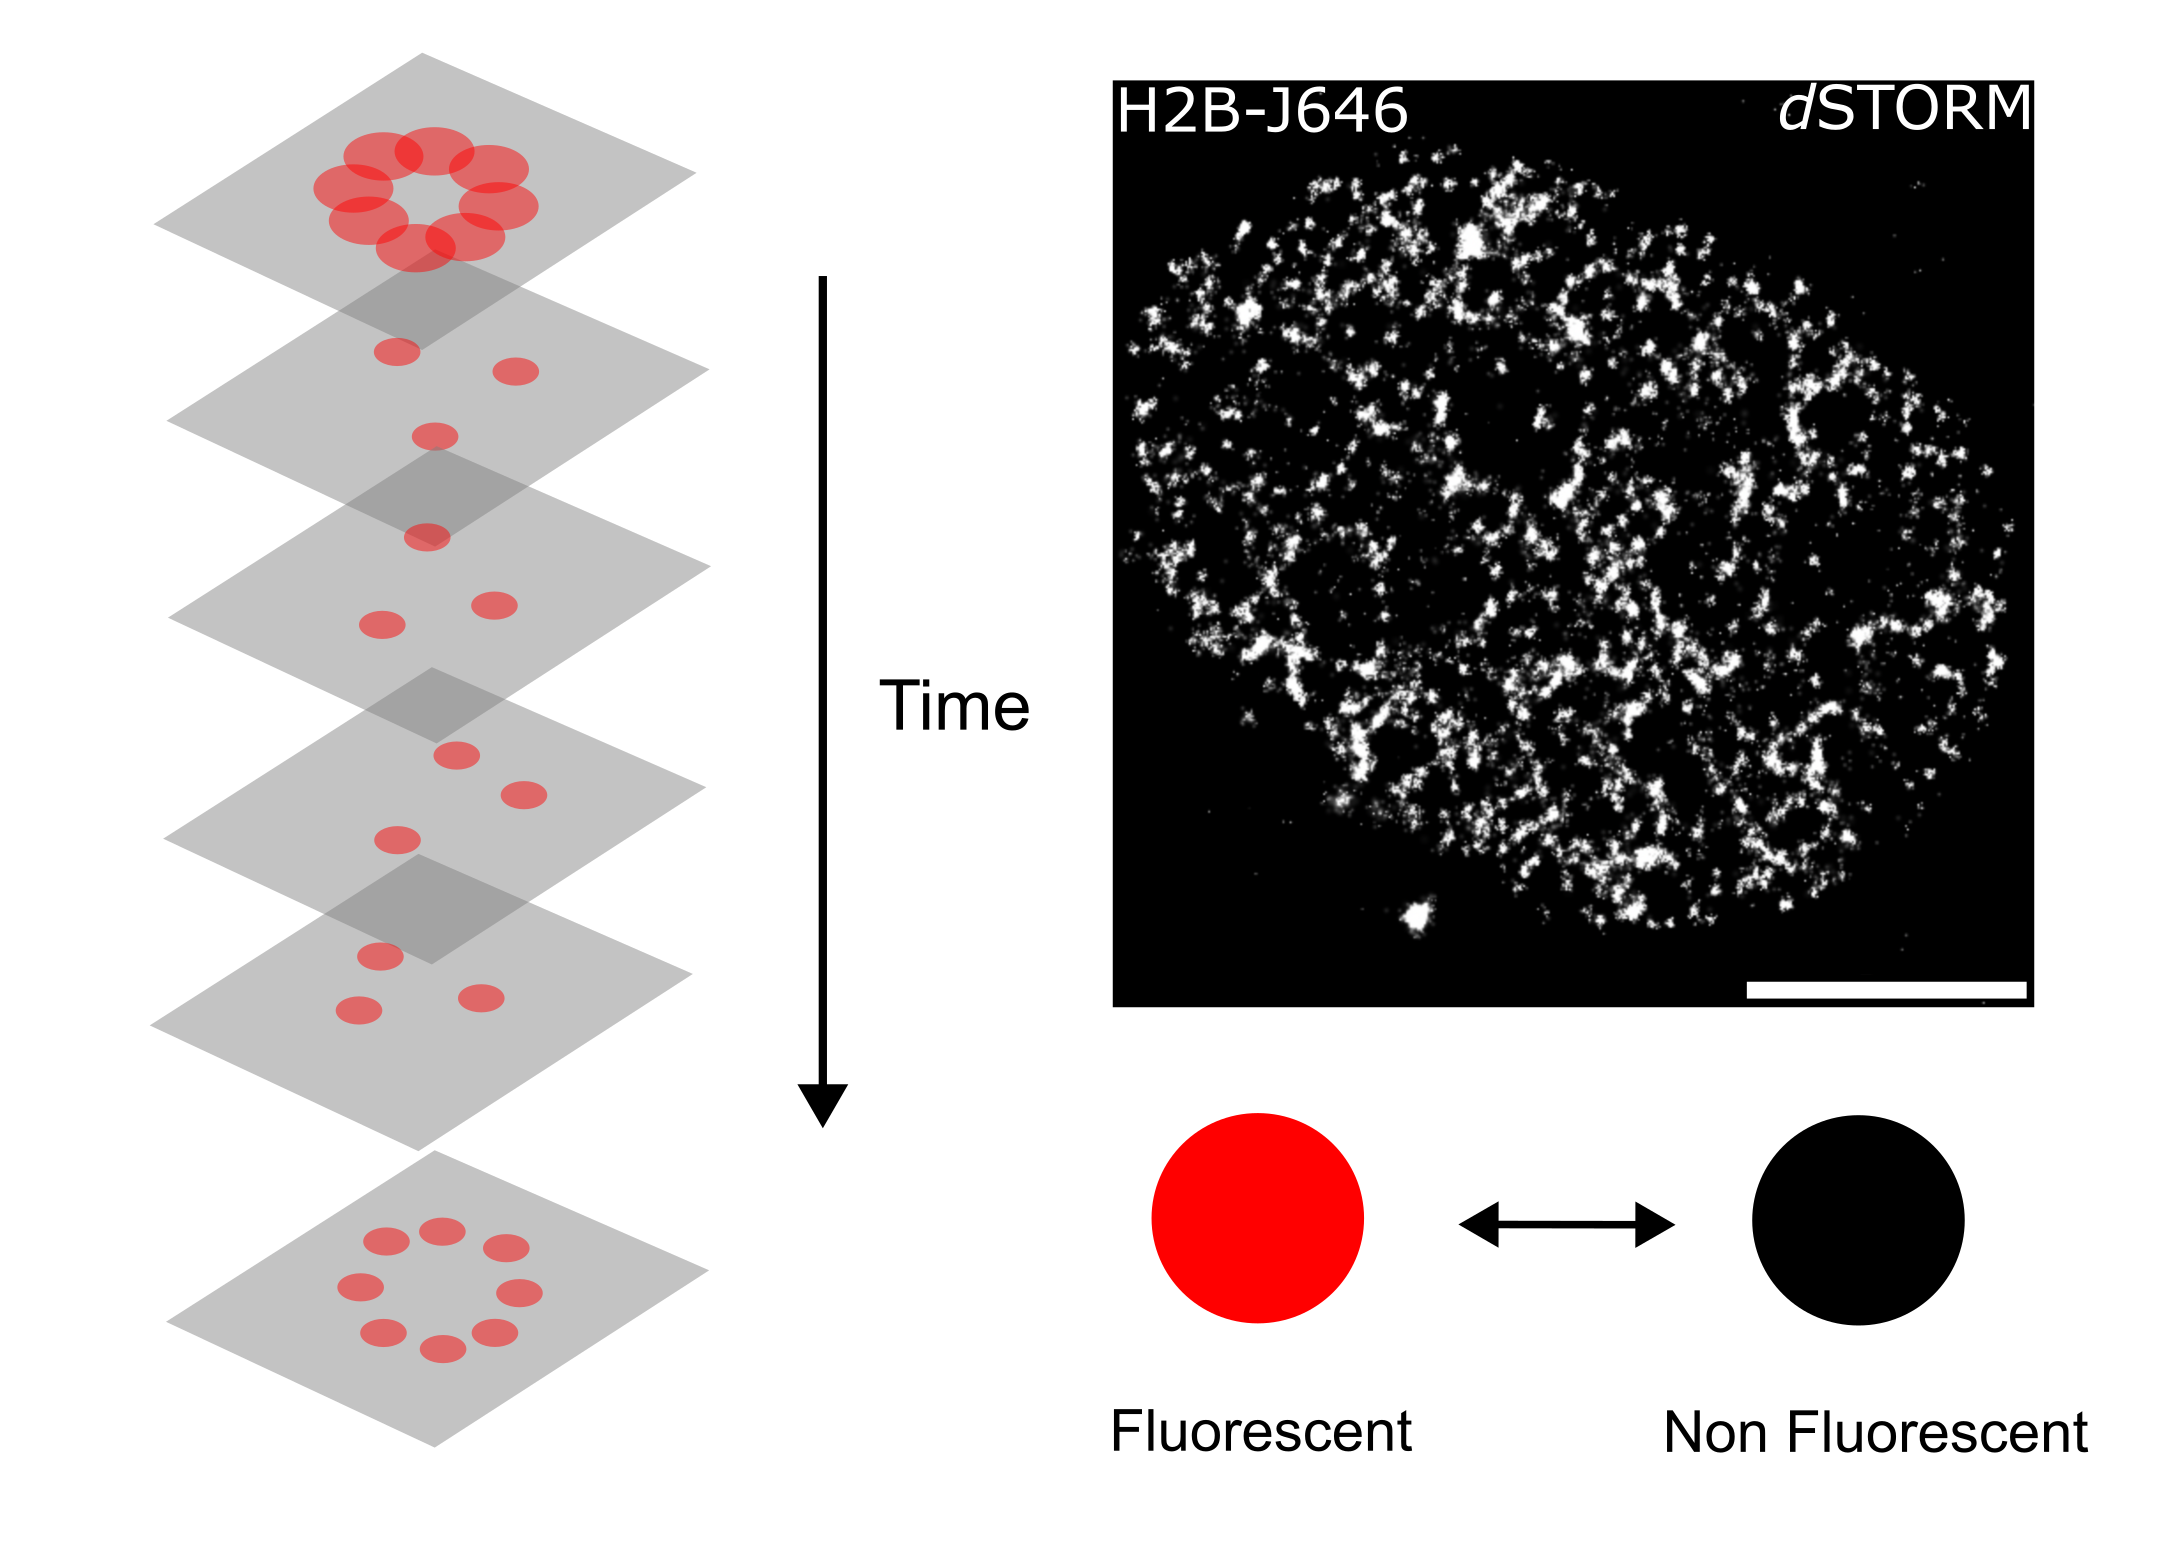
\includegraphics[width=12cm]{media/Intro.png}
\caption{\textbf{Stochastic optical reconstruction microscopy (STORM)}. (A) Single molecules are resolved by separating their fluorescent emission in time, using fluorophores with multiple photophysical states (B) Example super-resolution image of H2B protein in a living Hela cell nucleus at 37C, 5 percent CO2. Image reconstructed from $10^{3}$ 10ms frames. Scalebar 5um.}
\end{figure}

\begin{figure}[t]
\centering
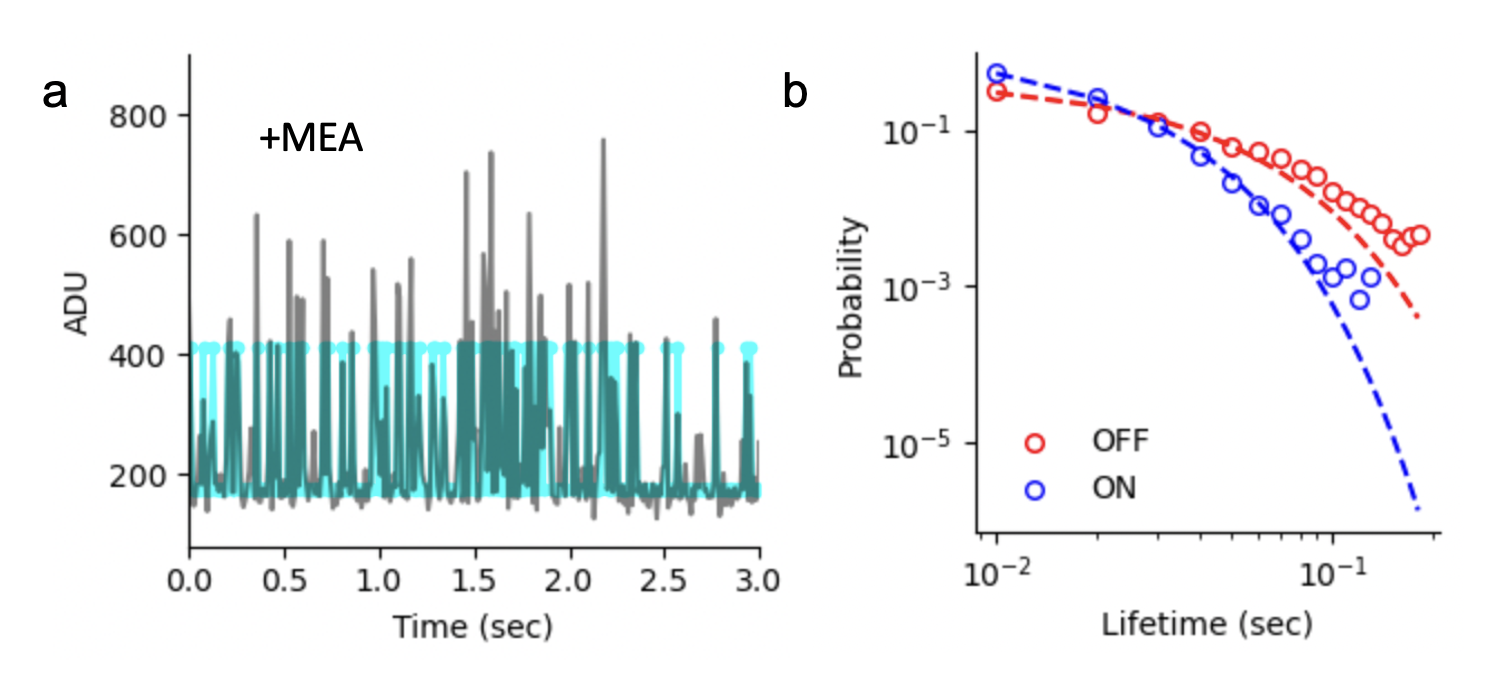
\includegraphics[width=13cm]{media/Lifetime.png}
\caption{Photoswitching of JF646 bound to H2B-HaloTag. (a) Peak intensity fluctuations of a putatively isolated JF646 molecule exicted at 640nm and imaged with 10ms exposure time in the presence of 100mM MEA buffer. Fit of a Poisson HMM is shown in cyan (b) ON and OFF state lifetime distributions found by pooling data from 16 JF646 spots in a single HeLa cell nucleus. Single component exponential fits shown as solid lines.}
\end{figure}


\section{The Image Likelihood}

It is common to describe the optical impulse response of a microscope as a two-dimensional isotropic Gaussian \parencite{Zhang2007}. This is an approximation to the more rigorous diffraction models given by \parencite{Richards1959,Gibson1989}. Over a continuous domain, the impulse response reads

\begin{equation*}
O(u,v) = \frac{1}{2\pi\sigma_{\bold{x}}^{2}}e^{-\frac{(u-\theta_{u})^{2}+(v-\theta_{v})^{2}}{2\sigma_{\bold{x}}^{2}}}
\end{equation*}

The above expression can be interpreted as a probability distribution over locations where a photon can be detected. Therefore, for discrete detectors, we discretize this expression by integrating over pixels. The number of photon arrivals will follow Poisson statistics, with expected value

\begin{equation*}
\mu_{k} = i_{0}\left(\int_{u_{k}-\delta /2}^{u_{k}+\delta /2} O(u; \theta_{u})du \right)\left(\int_{v_{k}-\delta /2}^{v_{k}+\delta /2} O(v;\theta_{v})dv \right)
\end{equation*}

The scalar quantity $i_{0}$ represents the amplitude of the signal, which is proportional the quantum efficiency of a pixel $\eta$, the duration of exposure, $\Delta$, and the number of photons emitter by a fluorescent molecule $N_{0}$. With no loss of generality, $\Delta = \eta = 1$ and there is a single free parameter $N_{0}$. Terms above in parentheses are simply integrals of Gaussian functions and can be evaluated analytically. I define them as $\Gamma_{u},\Gamma_{v}$, respectively. For example,

\begin{align*}
\Gamma_{u} &\vcentcolon  \int_{0}^{u_{k}+\delta /2 - \theta_{u}} O(u)du - \int_{0}^{u_{k}-\delta /2 - \theta_{u}} O(u)du\\
&= \frac{1}{2}\left(\mathrm{erf}\left(\frac{u_{k}+\frac{\delta}{2}-\theta_{i}}{\sqrt{2}\sigma_{\bold{x}}}\right) -\mathrm{erf}\left(\frac{u_{k}-\frac{\delta}{2}-\theta_{i}}{\sqrt{2}\sigma_{\bold{x}}}\right)\right)
\end{align*}

where we have used the common definition $\mathrm{erf}(z) = \frac{2}{\sqrt{\pi}}\int_{0}^{z}e^{-t^{2}}dt$. Recall the central objective of SMLM is to infer a set of molecular coordinates $\theta=(\theta_{u},\theta_{v})$ from measured low resolution images $\bold{x}$. In general, the likelihood on a particular pixel $p(\bold{x}_k\lvert\theta)$ is taken to be a convolution of Poisson and Gaussian distributions, due to shot noise $p(s_{k}) = \mathrm{Poisson}(\mu_{k})$ and sensor readout noise $p(\xi_{k}) = \mathcal{N}(o_{k},w_{k}^{2})$ 

\begin{figure}[t]
\begin{center}
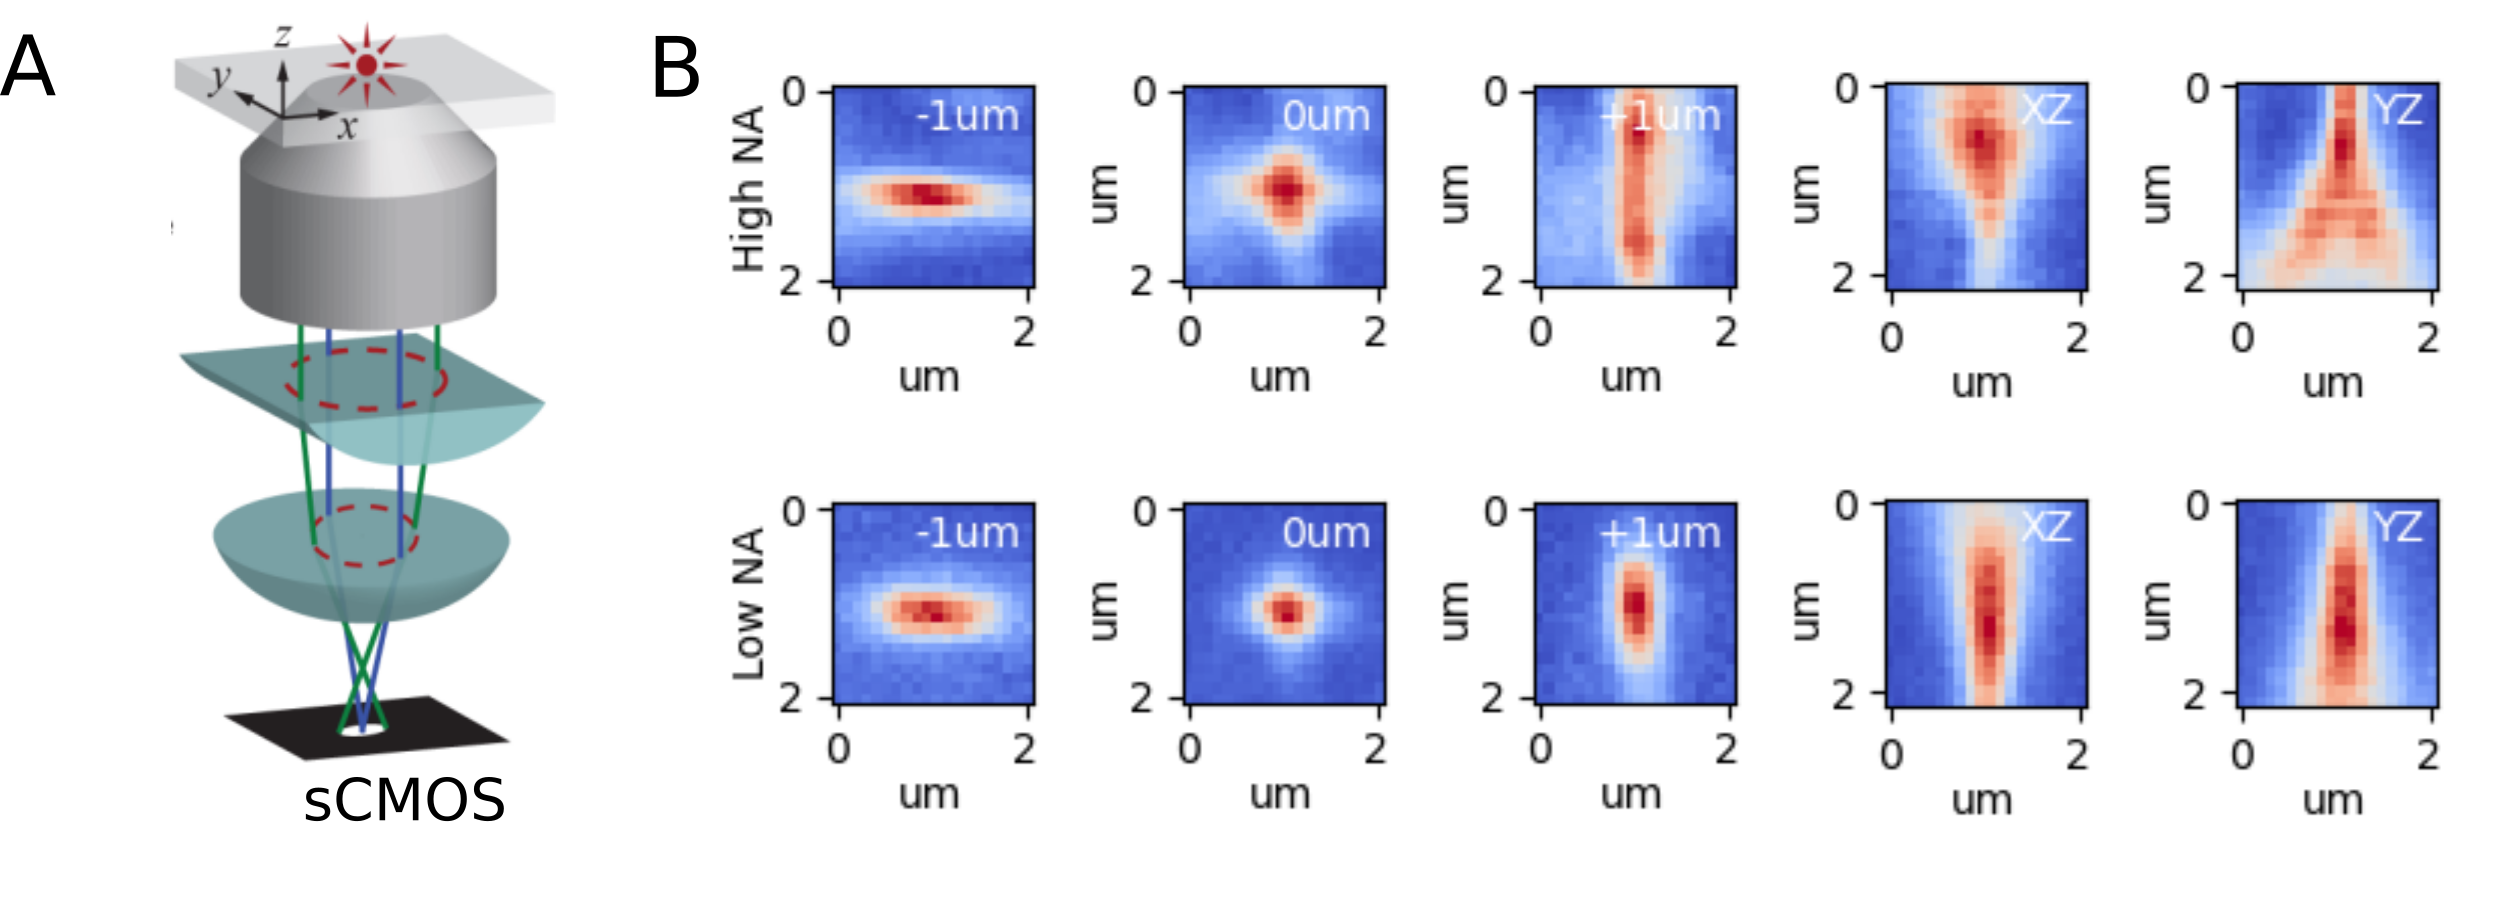
\includegraphics[width=14cm]{media/Astigmatism-Crop.png}
\end{center}
\caption{}
\end{figure}


\begin{figure}[t]
\begin{center}
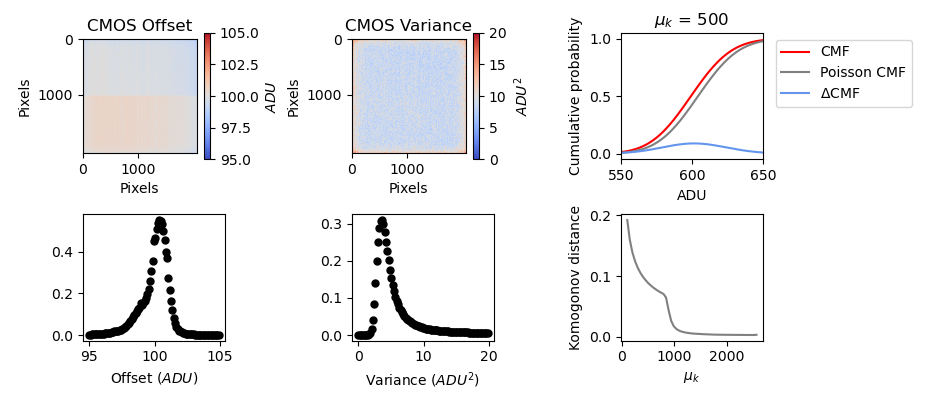
\includegraphics[width=16cm]{media/Noise.png}
\end{center}
\caption{\textbf{Noise model for CMOS cameras used for MLE}. (left)) CMOS offset for zero incident photons (middle) CMOS variance for zero incident photons (upper right) Cumulative mass function for the convolution distribution and its Poisson approximation for rate parameter $\mu_{k} = 500$ counts (lower right) Komogonov distance measured as a function of rate parameter $\mu_{k}$}
\end{figure}


\begin{equation}
p(\bold{x}_{k}\lvert\theta) = A\sum_{q=0}^{\infty} \frac{1}{q!}e^{-\mu_{k}}\mu_{k}^{q}\frac{1}{\sqrt{2\pi}w_{k}}e^{-\frac{(\bold{x}_{k}-g_{k}q-o_{k})^2}{2 w_{k}^{2}}} \approx \mathrm{Poisson}(\mu_{k}')
\end{equation}

where $A$ is some normalization constant. For the sake of generality, we include a per-pixel gain factor $g_{k}$, which is often unity. Sampling from $p(\bold{x}_{k}\lvert\theta)$ is trivial; however, for computation of a lower bound on uncertainty in $\theta$, the summation in (1) can be difficult to work with. Therefore, we choose to use a Poisson approximation for simplification, valid under a range of experimental conditions (Huang2013). After subtraction of a known offset $o_{k}$ of the pixel array, which can be easily measured, we have $\mu_{k}' = \mu_{k} + w_{k}^{2}$.

Under the Poisson approximation in the likelihood, the model negative log-likelihood is

\begin{equation}
\ell(\bold{x}\lvert\theta) = -\log \prod_{k} \frac{e^{-\left(\mu_{k}'\right)}\left(\mu_{k}'\right)^{n_{k}}}{n_{k}!} = \sum_{k}  \log n_{k}! + \mu_{k}' - n_{k}\log\left(\mu_{k}'\right)
\end{equation}

Localization then proceeds by minimization of $\ell(\bold{x}\lvert\theta)$. 


\subsection{Maximization of density, minimization of error}

\begin{figure}[t]
\begin{center}
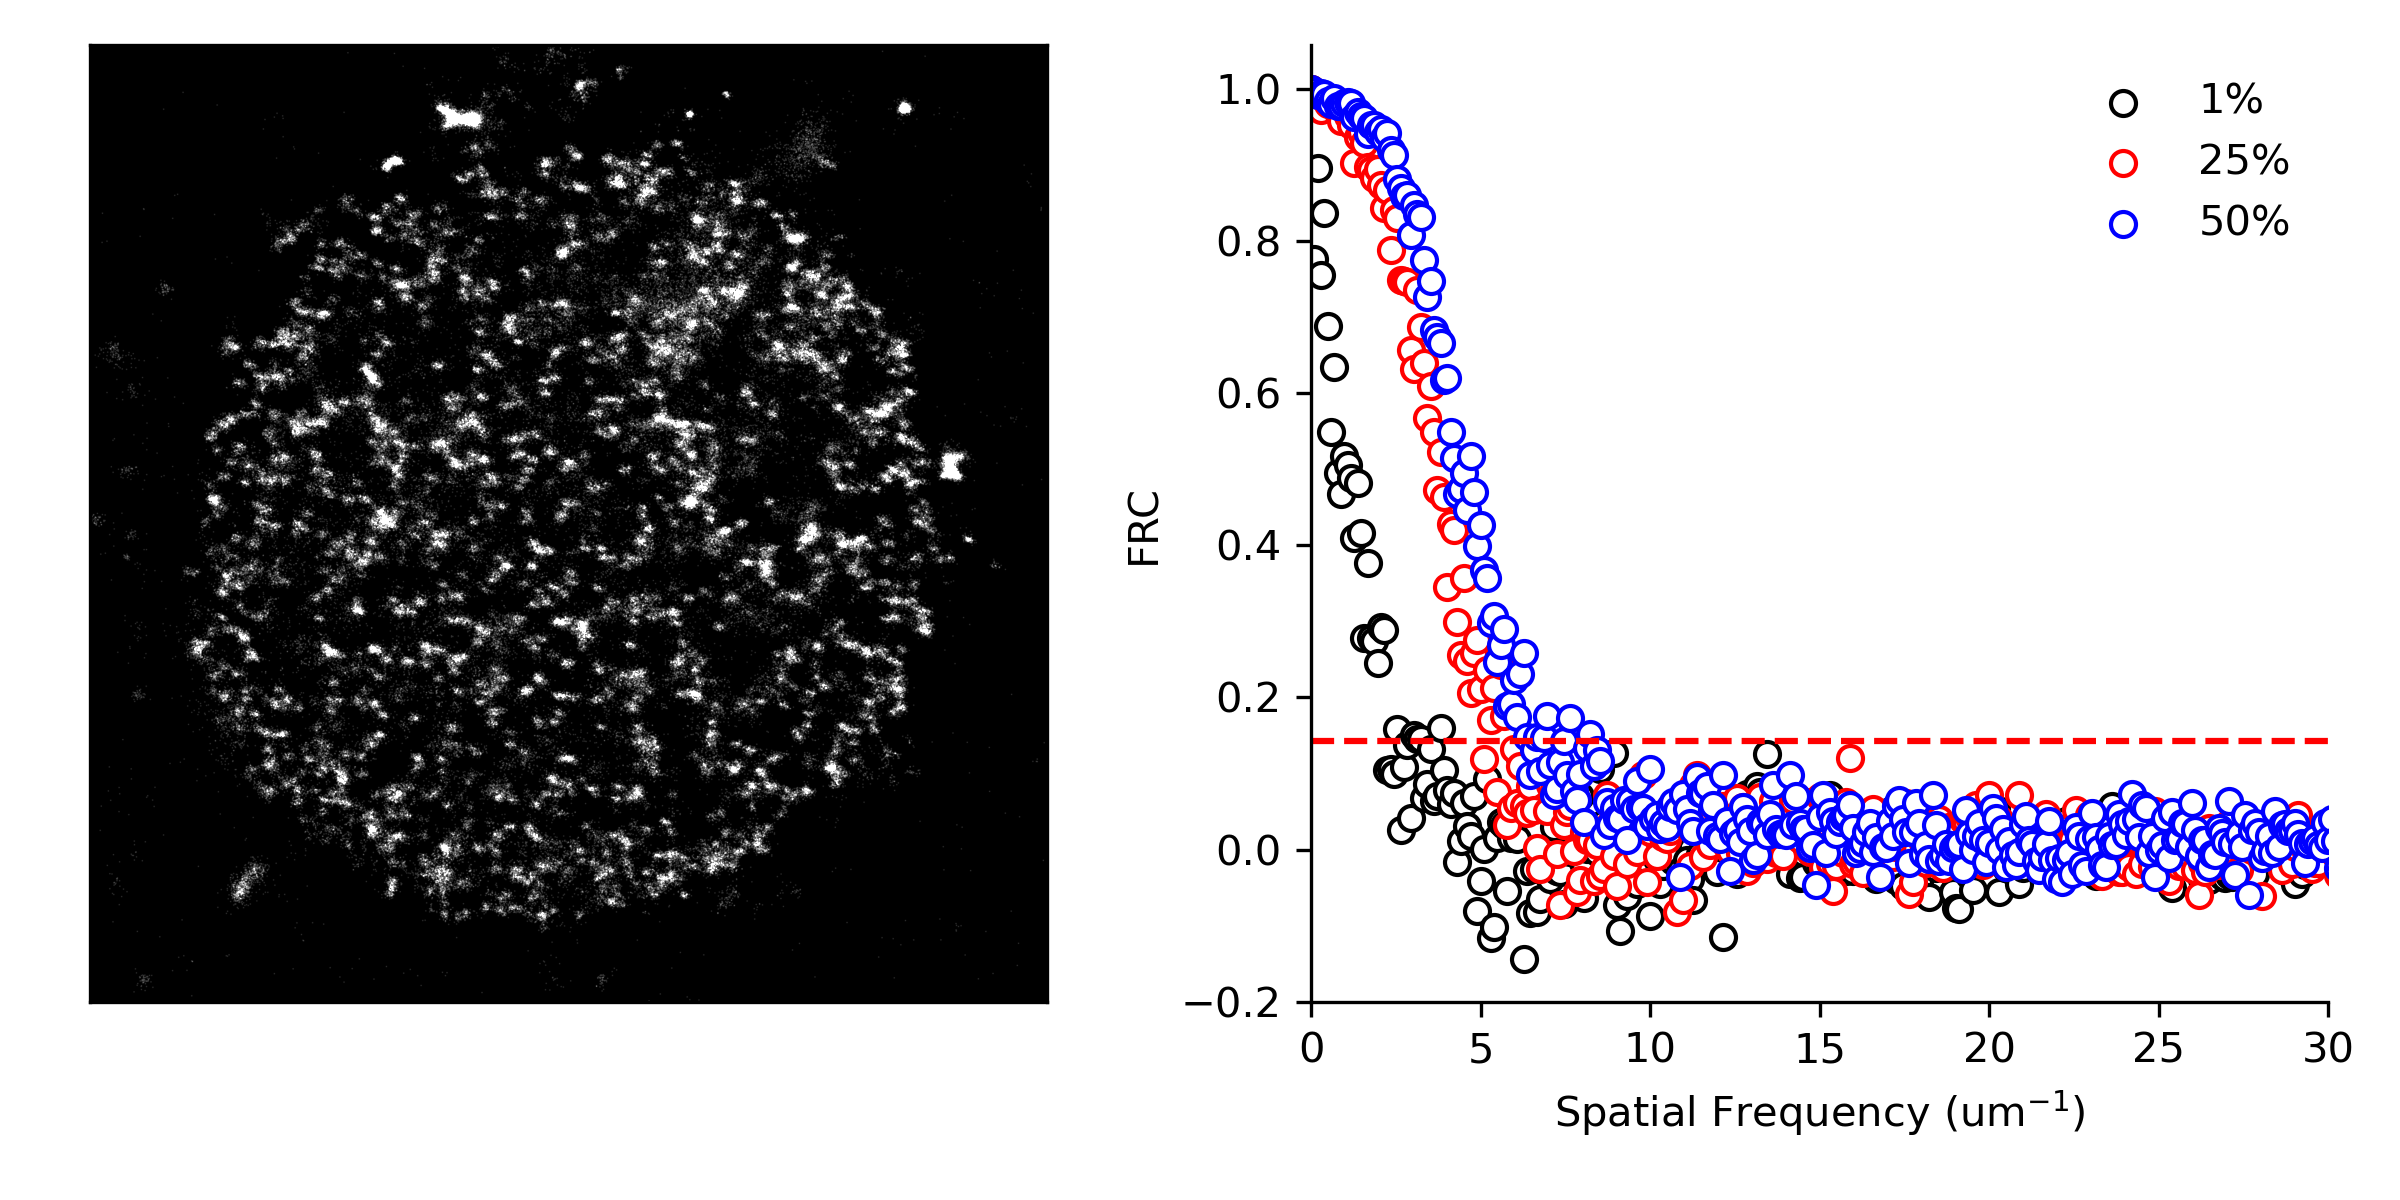
\includegraphics[width=14cm]{media/FRC.png}
\end{center}
\caption{\textbf{Noise model for CMOS cameras used for MLE}. (left)) CMOS offset for zero incident photons (middle) CMOS variance for zero incident photons (upper right) Cumulative mass function for the convolution distribution and its Poisson approximation for rate parameter $\mu_{k} = 500$ counts (lower right) Komogonov distance measured as a function of rate parameter $\mu_{k}$}
\end{figure}


The distribution of a particular biomolecule in the cell can be described as a probability density over a two-dimensional space, casting super-resolution as a density estimation problem. Intuitively, the spatial resolution of SMLM images then increases as we draw more samples from this density - a concept which is made mathematically precise by the so-called Fourier ring correlation or FRC. Using FRC, one can compute image resolution as the spatial frequency at which a correlation function in the frequency domain drops below a threshold, typically taken to be $1/7$ (See Supplement). According to this theory, reducing localization uncertainty while increasing the number of samples, results in an increase in image resolution (Nieuwenhuizen 2013). However, there remains a fundamental limit to the the minimal localization uncertainty which can be obtained.


\begin{equation*}
\mathrm{FRC}(q) = \frac{\sum_{\vec{q}\in\mathrm{circle}}\tilde{f_{1}}(\vec{q})\tilde{f_{2}}(\vec{q})^{*}}{\sqrt{\sum_{\vec{q}\in\mathrm{circle}}\lvert f_{1}(\vec{q})\lvert^{2}}\sqrt{\sum_{\vec{q}\in\mathrm{circle}}\lvert f_{2}}(\vec{q})\lvert^{2}}
\end{equation*}


Localization uncertainty, typically the RMSE of a maximum likelihood or similar statistical estimator, is bounded from below by the inverse of the Fisher information matrix, known as the Cramer-Rao lower bound (Chao 2016). Localization uncertainties in sparse conditions are often tens of nanometers, although recent work on integration of Bayesian priors with modulation enhanced SMLM (meSMLM) or structured illumination with MINFLUX, has reduced spatial resolution below to a few nanometers (Kalisvaart 2022, Gwosh 2020). Nevertheless, managing the increase in localization uncertainty at high labeling density remains a major bottleneck to SMLM. Static uncertainty due to molecular crowding can be partially amelioriated by using pairwise or higher-order temporal correlations within a pixel neighborhood, known as stochastic optical fluctuation imaging or SOFI (Dertinger 2009). Other approaches such as stimulated emission and depletion (STED) imaging bring control over the photophysical state of a chosen subset of the sample, yet the need for laser scanning prevents widespread application in live-cell studies. The spatial resolution and relative simplicity of SMLM techniques remains unmatched, inciting an effort to increase the resolution of SMLM techniques and explore avenues towards time resolved SMLM.

\subsection{Thesis}

To address the challenges posed by high-dimensional data in fluorescence nanoscopy, I propose two different methods:

The first method is model-heavy and leverages deep learning techniques. Specifically, it involves a generative modeling framework for kernel density estimation in single molecule localization microscopy, using variational diffusion. This approach not only accelerates super-resolution imaging but also provides a way to estimate uncertainty in the results.

The second method is model-light but relies on advanced hardware. This approach uses single photon avalanche diode (SPAD) arrays to accurately count active fluorescent emitters while performing intensity-based multi-emitter localization. SPAD cameras, with their high temporal resolution and single photon sensitivity, enable precise localization in non-sparse scenes.

These two methods, one focusing on sophisticated computational models and the other on cutting-edge hardware, offer complementary solutions to the high-dimensional inference problem in super-resolution microscopy. By combining these approaches, we can achieve more accurate and reliable imaging of biological structures at the nanoscale.

